\subsection{Ergebnisse}

\subsubsection*{Übersicht}

\begin{longtable}{|l|l|c|}
    \hline
                        &           & \textbf{Anzahl} \\ \hline
    Teilnehmer          & insgesamt & 9745 \\
                        & gefiltert & 4015 \\ \hline
    Gefahrene Routen    & insgesamt & 41540 \\
                        & gefiltert & 16531 \\ \hline
\caption{}
\label{tab:study_user_overview}
\end{longtable}

Um bei der Analyse der Daten, Nutzer auszuschließen, die eine Navigation nur gestartet haben, um sich diese anzusehen, aber NUNAV nicht aktiv während einer Autofahrt genutzt haben werden Routen, die kürzer als 4 Kilometer sind herausgefiltert. Dies verhindert außerdem, dass das gelangen zur ersten Route, sowie das Suchen von Parkplätzen einen zu großen Einfluss auf die Daten hat.

\subsubsection{Einfluss der Erklärungen}

\textbf{Nutzerabweichungen von der vorgeschlagenen Route}

\textbf{Hypothesen}

\begin{enumerate}
    \item Wenn der Nutzer Erklärungen erhält, dann folgt er signifikant häufiger der vorgeschlagenen Route als wenn er keine erhält.
    \item Wenn der Nutzer einen der beiden Erklärungstypen (Algorithmus, Navigation) erhält, dann folgt er signifikant weniger der vorgeschlagenen Route als wenn er beide erhält.
\end{enumerate}

 Als Messwert wird die Anzahl der \textit{Offroutes} relativ zu Gesamtlänge der Route verwendet. Die Einheit ist Offroute pro Kilometer.

\smallskip

\noindent\colorbox{lightgray}{%
    \parbox{0.975\linewidth}{
        \textbf{Definition}

        Ein \textit{Offroute} ist der Fall, dass der Nutzer sich aktuell nicht auf der vorgeschlagenen Route befindet. Konkret bedeutet dies, dass das Smartphone NUNAV eine neue Position bereitstellt und nach einer Evaluation bestimmter Kriterien festgestellt wird, dass sich der Nutzer nicht mehr auf der Route befindet. In der Regel wird dann eine neue Route vom Server angefordert.
        
        \textit{Zu Beachten}
        \begin{itemize}
            \item Bis der Nutzer eine neue Route erhält, kann es mehrere \textit{Offroutes} geben.
            \item Es kann sein, dass der Nutzer mehrfach wieder die gleiche Route erhält.
            \item Ein kann auch zu einem \textit{Offroute} kommen, wenn die Nutzerposition schlecht ist.
        \end{itemize}
    }
}

\smallskip

Bei der Betrachtung der \textit{Offroutes} werden zuerst Ausreißer herausgefiltert. (Ausreißer: mehr als 3 Standardabweichungen vom Durchschnitt entfernt). Folglich sind 16366 Routen im Datensatz für die Prüfung der Hypothese verblieben.

\begin{figure}[bth]!
    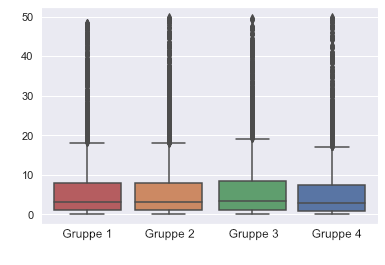
\includegraphics{contents/06_model_evaluation/res/OffRoute_Result_Overview.png}
    \caption{Anzahl der Offroutes pro Kilometer für jede Studiengruppe}
\end{figure}

\begin{longtable}{|c|c|c|c|}
    \hline
    \textbf{Studiengruppe}  & \textbf{Mittelwert} & \textbf{Median} & \textbf{Standardabweichung} \\ \hline
    Gruppe 1                & 7.85 & 3.27 & 13.75 \\ \hline
    Gruppe 2                & 8.20 & 3.30 & 14.30 \\ \hline
    Gruppe 3                & 7.90 & 3.57 & 12.81 \\ \hline
    Gruppe 4                & 7.48 & 2.90 & 13.74 \\ \hline
\caption{Übersicht der Ergebnisse der Routen-Abweichungen pro Kilometer}
\label{tab:study_offroute_results}
\end{longtable}

Um zu prüfen, ob die Unterschiede der Mittelwerte signifikant ist, muss dies mittels eines statistischen Tests überprüft werden. Da es sich um ein Experiment von mehren nicht zusammenhängenden Studiengruppen mit mehr als zwei verschiedenen Bedingungen handelt, kommen entweder ein ANOVA- oder Kruskal-Wallis-Test in Frage. Für ersteren gilt, dass die Daten gleich verteilt sein müssen. Dies wurde mittels Shapiro-Wilk-Test test geprüft. Da das Ergebnis für alle Test-Gruppen $ p = 0.000000 < 0.05 $ ist, sind die Daten nicht normal verteilt. Folglich wird zur Signifikanzprüfung der Kruskal-Wallis-Test verwendet. Aufgrund der Ergebnis von $ p = 0.000008 < 0.05 $, kann abgeleitet werden, dass ein Haupteffekt vorliegt.

Für die Prüfung zwischen welchen Studiengruppen ein signifikanter Unterschied vorliegt, wird der Dunn-Test \cite{dunn1964multiple} verwendet.

Dieser liefert folgende Ergebnisse:

\begin{longtable}{|c|c|c|c|c|}
    \hline
    & \textbf{Gruppe 1} & \textbf{Gruppe 2} & \textbf{Gruppe 3} & \textbf{Gruppe 4} \\ \hline
    \textbf{Gruppe 1}   & 1.000000 & 1.000000 & 0.219884 & 0.008222 \\ \hline
    \textbf{Gruppe 2}   & 1.000000 & 1.000000 & 0.860586 & 0.000912 \\ \hline
    \textbf{Gruppe 3}   & 0.219884 & 0.860586 & 1.000000 & 0.000005 \\ \hline
    \textbf{Gruppe 4}   & 0.008222 & 0.000912 & 0.000005 & 1.000000 \\ \hline

    \caption{Signifikanzniveau $ p $ im paarweisen Vergleich der Anzahl der Routenabweichungen pro Kilometer zwischen den Studiengruppen }
    \label{tab:study_offroute_significance_results}
\end{longtable}

Auch hier wird wieder von einem Signifikanzniveau $ p < 0.05 $ ausgegangen. Folglich weichen die Nutzer der Gruppe 4 signifikant weniger von der vorgeschlagenen Route ab im Vergleich zu allen anderen Gruppen. Weitere signifikante Unterschiede lassen sich nicht erkennen.

Hypothese 1 trifft zwar für das Geben aller Erklärungstypen (Gruppe 4) zu, nicht aber für die Gruppen 2 und 3. Folglich wird Hypothese 1 abgelehnt.  Hypothese 2 hat sich vollumfänglich als richtig erwiesen, da die Nutzer der Gruppe 4 sowohl signifikant weniger von der vorgeschlagenen Route abgewichen sind also auch signifikant weniger als die Nutzer der Gruppe 2.

\textbf{Häufigkeit der Nutzung}

\textbf{Hypothesen}

\begin{enumerate}
    \item Wenn der Nutzer Erklärungen erhält, dann verwendet er NUNAV signifikant häufiger, als wenn er keine erhält.
    \item Wenn der Nutzer einen der beiden Erklärungstypen (Algorithmus und Navigation) erhält, dann nutzt er NUNAV signifikant seltener als wenn er beide erhält.
\end{enumerate}

Als Messwert wird die Anzahl der gefahrenen Routen genommen.

Bei der Betrachtung der Anzahl der gefahrenen Routen werden zuerst Ausreißer herausgefiltert. (Ausreißer: mehr als 3 Standardabweichungen vom Durchschnitt entfernt). Folglich sind 3954 Nutzer im Datensatz für die Prüfung der Hypothesen verblieben.

\begin{figure}[bth]!
    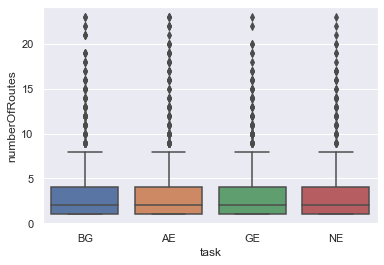
\includegraphics{contents/06_model_evaluation/res/Usage_Result_Overview.png}
    \caption{Anzahl der gefahrenen Routen für jede Studiengruppe}
\end{figure}

\begin{longtable}{|c|c|c|c|}
    \hline
    \textbf{Studiengruppe}  & \textbf{Mittelwert} & \textbf{Median} & \textbf{Standardabweichung} \\ \hline
    Gruppe 1                & 3.43 & 2.0 & 3.49 \\ \hline
    Gruppe 2                & 3.69 & 2.0 & 3.86 \\ \hline
    Gruppe 3                & 3.42 & 2.0 & 3.47 \\ \hline
    Gruppe 4                & 3.57 & 2.0 & 3.44 \\ \hline
\caption{Übersicht der Ergebnisse der gefahrenen Routen der Nutzer}
\label{tab:study_offroute_results}
\end{longtable}

Um zu prüfen, ob die Unterschiede der Mittelwerte signifikant ist, muss dies mittels eines statistischen Tests überprüft werden. Da es sich um ein Experiment von mehren nicht zusammenhängenden Studiengruppen mit mehr als zwei verschiedenen Bedingungen handelt, kommen entweder ein ANOVA- oder Kruskal-Wallis-Test in Frage. Für ersteren gilt, dass die Daten gleich verteilt sein müssen. Dies wurde mittels Shapiro-Wilk-Test test geprüft. Da das Ergebnis für alle Test-Gruppen $ p = 0.000000 < 0.05 $ ist, sind die Daten nicht normal verteilt. Folglich wird zur Signifikanzprüfung der Kruskal-Wallis-Test verwendet. Aufgrund des Ergebnisses von $ p = 0.197473 > 0.05 $, kann abgeleitet werden, dass kein Haupteffekt vorliegt.

Da es keine signifikanten Ergebnisse gibt müssen beide Hypothesen abgelehnt werden.

Bemerkung: Ich habe hier die durchschnittliche Anzahl der Routen pro Nutzer untersucht. Was aber, wenn ein Nutzer aufhört NUNAV zu benutzen während dem Test? Ich werde also noch die Gesamtzahl der gefahrenen Routen pro Nutzergruppe vergleichen. Das schicke ich dir dann Anfang der Woche.

\textbf{Nutzerzufriedenheit mit der aktuellen Route}

\textbf{Hypothesen}

\begin{enumerate}
    \item Wenn der Nutzer Erklärungen erhält, dann ist er zufriedener mit der Navigation.
    \item Wenn der Nutzer einen der beiden Erklärungstypen (Algorithmus, Navigation) erhält, dann ist er weniger zufrieden mit der Navigation als wenn er beide erhält.
\end{enumerate}

Als Messwert wird eine Likert-Skala, auf der der Nutzer in Form von fünf Sternen bewerten kann, wie gut ihm die abgeschlossene Navigation gefallen hat. 

\begin{figure}[bth]!
    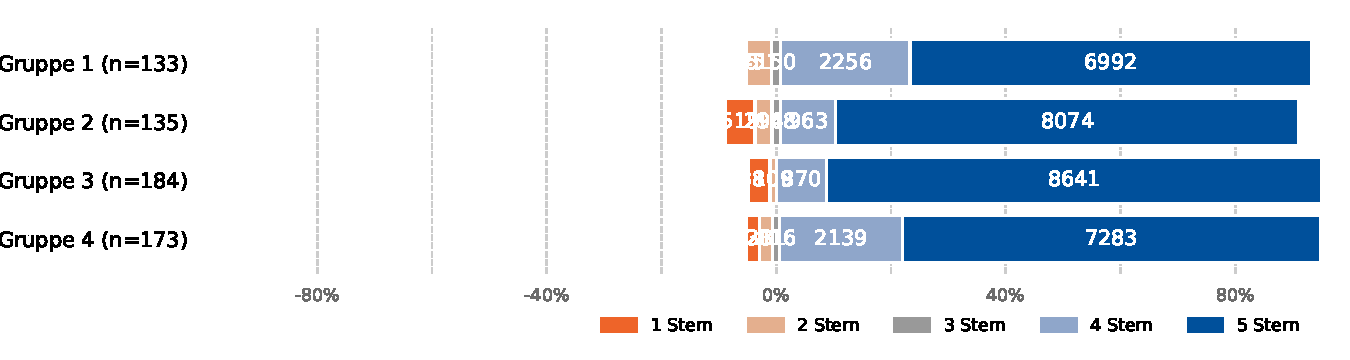
\includegraphics[width=\linewidth]{contents/06_model_evaluation/res/Rating_Result_Overview.pdf}
    \caption{Durchschnittliche Bewertung der Navigation pro Nutzer  für jede Studiengruppe}
\end{figure}

Für die Prüfung zwischen welchen Studiengruppen ein signifikanter Unterschied vorliegt, wird wieder der Dunn-Test \cite{dunn1964multiple} verwendet. (P wird mit der \glqq bonferoni\grqq{}-Methode korrigiert.)

Dabei kommt heraus, dass es zwischen den Gruppen 1 und 2 ($ p = 0.003027$) sowie 1 und 4 ($ p = 0.0.034375 $) einen signifikanten Unterschied gibt. Außerdem gibt es einen signifikanten Unterschied zwischen Gruppe 2 und 3 ($ p = 0.021798 $). Zusammen mit den Ergebnissen der Likert Skala, kann man also sagen, dass die Zufriedenheit der Nutzer im Vergliech zu keinen Erklärungen besser ist, wenn die Erklärungen wie in Gruppe 4 gegeben werden. Und Es kann gesagt werden, dass die Zufriedenheit bei Gruppe 2 gegenüber Gruppe 3 höher ist sowie bei Gruppe 1 gegenüber Gruppe 4. In letzterem Fall hat sich die Zufriedenheit beim Geben von Erklärungen folglich sogar verschlechtert.

Da beim Geben von Erklärungen dies die Nutzerzufriedenheit nicht in jedem Fall erhöht, muss Hypothese 1 abgelehnt werden. Hypothese 2 muss ebenfalls abgelehnt werden, da es keine signifikanten Zusammenhänge zwischen den Gruppen 2 und 4 bzw. 3 und 4 gibt.

Bemerkung: Hier muss ich noch mit der Anzahl der Nutzer normalisieren. Dann könnte ein Effekt auftreten.